\documentclass[12pt]{article}

\usepackage[utf8]{inputenc}
\usepackage{mhchem}
\usepackage{chemfig}
\usepackage{fancyhdr}
\usepackage{grapicx}

\title{Kemiaflevering 14}
\author{Jeppe Møldrup}
\date{}

\pagestyle{fancy}
\fancyhead[L]{Jeppe Møldrup}
\fancyhead[C]{Kemi 14}
\fancyhead[R]{08/04-2019}

\begin{document}

\maketitle{}

\section*{Opgave 2}

d.

Jeg ved at K afhænger af gibbs energi i formlen
$$-\Delta G^{\circ} = R\cdot T\cdot ln K$$
Så jeg finder først gibbs energi ved $260^{\circ} = 533.15\ K$ med formlen fra b
$$-\Delta G^{\circ}(533.15\ K) = 12.35\ kJ\cdot mol^-1$$
Så isolerer jeg K
$$-\Delta G^{\circ} = R\cdot T\cdot ln K \Leftrightarrow K = e^{\frac{-\Delta G^{\circ}}{R\cdot T}}$$
Og indsætter
$$K = e^{\frac{12.35\ kJ\cdot mol^-1}{8.314\cdot 533.15}} = 16.26\ bar$$
K har enheden bar ud fra ligevægtsbrøken.

e.

Jeg opstiller et STL-skema med partialtryk i stedet for mol, idet
partialtrykket er proportionalt med stofmængden

\begin{center}
        \begin{tabular}{| c | c | c | c | c | c |}
                \hline
                & 2-Chlor-2-methylpropan & \ce{<=>} & 2-methylprop-1-en & + & Cl \\ \hline
                Start & x & & 0 bar & & 0 bar \\ \hline
                Tilvækst & -0.52 bar & & 0.52 bar & & 0.52 bar \\ \hline
                Slut & x-0.52 bar & & 0.52 bar & & 0.52 bar \\ \hline
        \end{tabular}
\end{center}

Så kan jeg finde partialtrykket af 2-Chlor-2-methylpropan til slut med ligevægtsbrøken
da jeg kender K-værdien fra sidste opgave.
$$solve(16.21\ bar=\frac{0.52\ bar \cdot 0.52\ bar}{x},x) \rightarrow x = 0.01668\ bar$$
Så kan jeg finde partialtrykket ved start ved at lægge 0.52 bar til idet(se STL-skema)
$$0.01668\ bar + 0.52\ bar = 0.53668\ bar$$
Så kan jeg isolere stofmængde i idealgasligningen
$$pV = nRT \Leftrightarrow n = \frac{PV}{RT}$$
og indsætte
$$n = \frac{0.53668\ bar \cdot 3\ L}{0.0831\ bar\cdot L \cdot mol^{-1}\cdot K^{-1}\cdot 533.15\ K} = 0.03634\ mol$$
Så ganger jeg med den molare masse af 2-Chlor-2-methylpropan
$$0.03634\ mol \cdot 92.57\ g/mol = 3.36\ g$$
Så massen af 2-Chlor-2-methylpropan er 3.36 g

\section*{Opgave 3}

c.\\
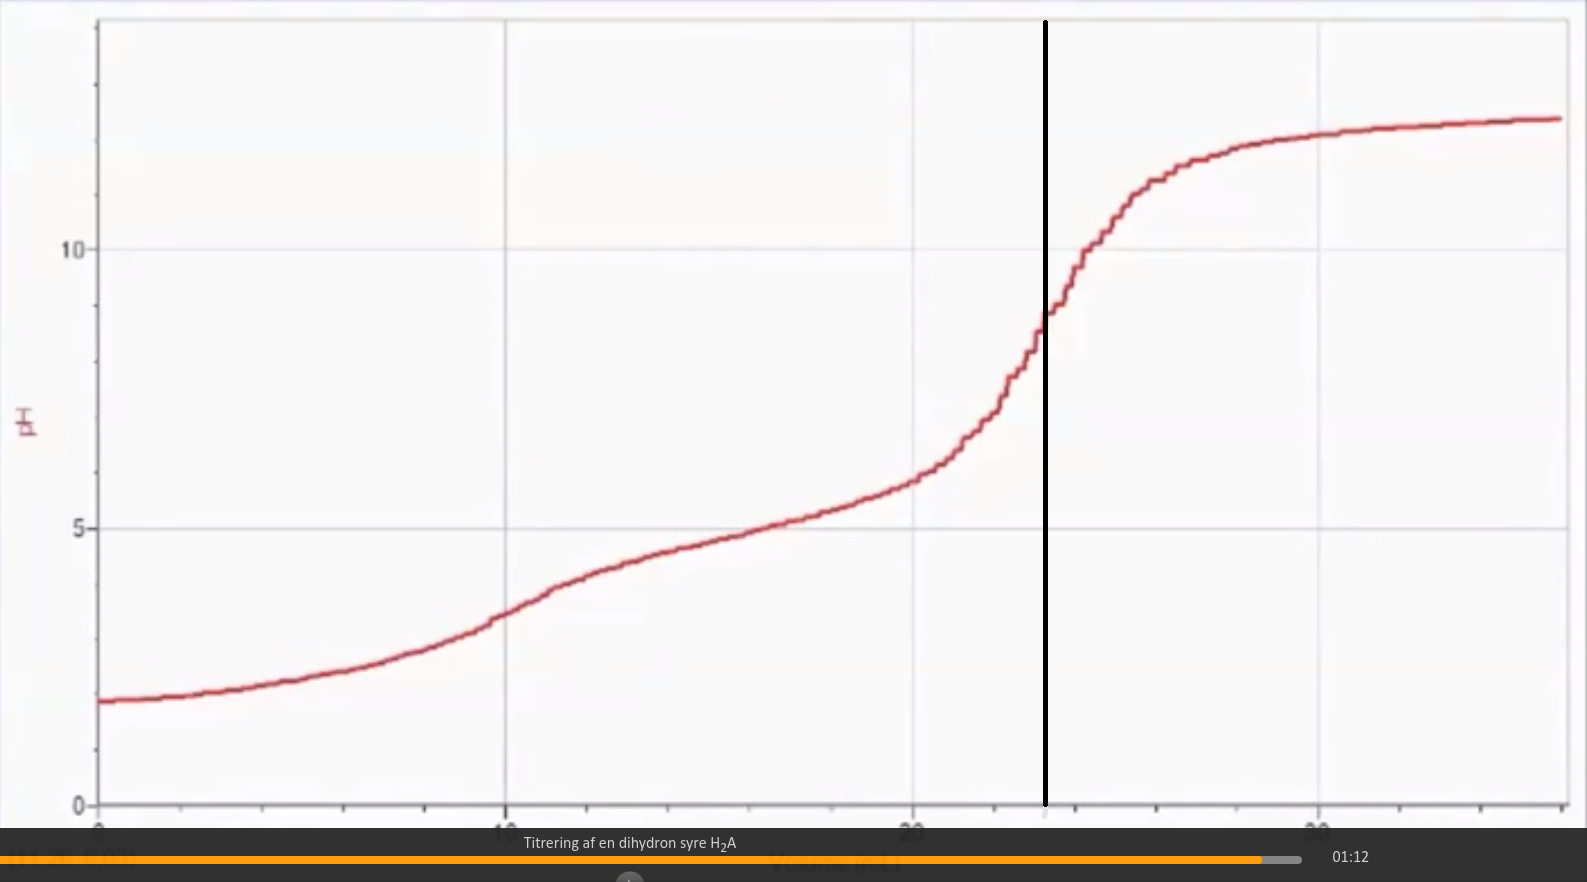
\includegraphics[width=\textwidth]{screenshot.png}
Massen af \ce{H2A} er 0.210 g. Der bliver hældt cirka 23.2 mL 0.124 M NaOH i før ækvivalænspunktet nåes. Så det svarer til
$$n(NaOH) = 0.124\ M \cdot 0.0232\ L = 0.0028768\ mol$$
Idet \ce{H2A} er en dihydron syre, vil NaOH reagerer med det i forholdet 2:1, dvs. stofmængden af \ce{H2A} er halvt så meget som
NaOH og derfor kan jeg finde den molare masse af \ce{H2A}
$$M(H_2 A) = \frac{0.210\ g}{0.0028768\ mol \cdot 0.5} \approx 146\ g/mol$$
Så den molare masse af stoffet er 146 g/mol

d.

Et molekyle danner bundfald med fehlingsvæske hvis det er en aldehyd, mens en
keton ikke gør. begge type danner bundfald med hydrazin. Så derfor er mine to
strukturformler.\\
Aldehyd:\\
\begin{center}
\chemfig{H-[1]O-[-1](=[-2]O)-[1](-[-1](=[-2]O)-[1]O-[-1]H)-[2]-[1](=[2]O)-[-1]H}
\end{center}
Keton:\\
\begin{center}
\chemfig{H-[1]O-[-1](=[-2]O)-[1](-[-1](=[-2]O)-[1]O-[-1]H)-[2](=[3]O)-[1]}
\end{center}
Og de genererede spektrummer for de to molekyler er:\\
Aldehyd:\\
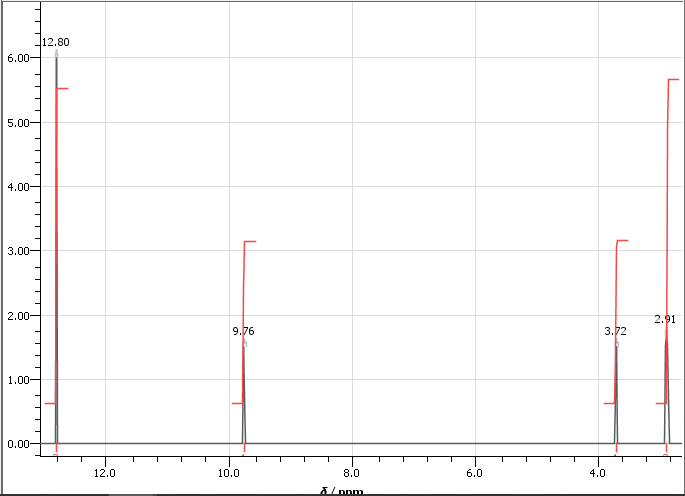
\includegraphics[width=\textwidth]{aldehyd.png}\\
Keton:\\
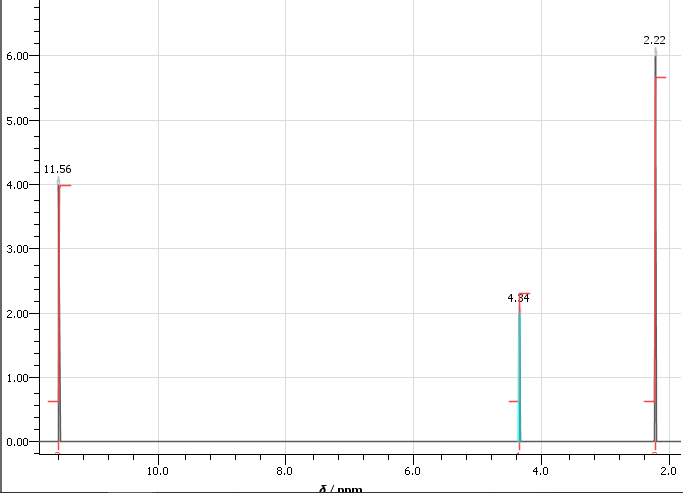
\includegraphics[width=\textwidth]{keton.png}

e.

Har ikke kunne finde den rigtige struktur

\end{document}
